\documentclass[12pt]{article}

\usepackage[utf8]{inputenc}
\usepackage{amsmath}
%\usepackage{ae}
\usepackage{graphicx}
\usepackage{color}
\usepackage{tikz}
%\usepackage{bbm}
%\usepackage[swedish]{babel}
\newcommand{\N}{\ensuremath{\mathbbm{N}}}
\newcommand{\Z}{\ensuremath{\mathbbm{Z}}}
\newcommand{\Q}{\ensuremath{\mathbbm{Q}}}
\newcommand{\R}{\ensuremath{\mathbbm{R}}}
\newcommand{\C}{\ensuremath{\mathbbm{C}}}
\newcommand{\rd}{\ensuremath{\mathrm{d}}}
\newcommand{\id}{\ensuremath{\,\rd}}
\newcommand{\ket}[1]{|#1\rangle}
\newcommand{\bra}[1]{\langle#1|}
\newcommand{\braket}[2]{\bra{#1}#2\rangle}
\newcommand{\bracket}[3]{\bra{#1}#2\ket{#3}}

\title{Holographic Superconductivity}
\author{Petter Säterskog}
\begin{document}
\maketitle
\tableofcontents

\section{Introduction}
\subsection{Background}
High TC Superconductors
Strong coupling
\subsection{The Conjecture}
The AdS-CFT correspondence was conjectured in 1997 \cite{Maldacena:1997re}. It relates the physics of a string theory in Anti de Sitter space (AdS) to a conformal field theory (CFT) on the boundary to the AdS space. The correspondence is given by the GKPW equation \cite{Witten:1998qj}
\begin{equation}
 Z_{\text{cft}}=Z_{\text{strings}}
\end{equation}
where $Z_{\text{cft}}$ is the partition function of the boundary theory and $Z_{\text{strings}}$ is the partition function of the bulk theory. The bulk partition function is in the classical limit
\begin{equation}
 Z_{\text{strings}}\propto\mathrm{e}^{-S_\text{extreme}}
\end{equation}
where $S_\text{extreme}$ is the extremal action and periodic Euclidean time is used. The boundary partition function can thus be calculated by finding the classical field configurations that extremize the action.
Describe generating functionals, the GKPW equation
\section{Application}
Classicallity
scalar example
show 4.68 from GKPW and classicallity assumption. Possible for general lagrangian?
\section{Application to Superconductor}
The Lagrangian used is
\begin{eqnarray}
 \mathcal{L}=&-\frac{1}{4}F_{ab}F^{ab}-m^2\psi\overline{\psi}-D_a\psi\overline{D^a\psi}
+\gamma C_{abcd}F^{ab}F^{cd}+\alpha_1(F_{ab}F^{ab})^2\nonumber\\
&+\alpha_2F^a_bF^b_cF^c_dF^d_a
\end{eqnarray}
where $D_a$ is the gauge covariant derivative $D_a=\nabla_a-iA_a$ and $F_{a,b}=\partial_aA_b-\partial_bA_a$. This Lagrangian is invariant under a U(1) gauge transformation
\begin{eqnarray}
 \psi&\rightarrow&\mathrm{e}^{i\theta(x)}\psi\\
 A_a&\rightarrow& A_a+\nabla_a\theta(x).
\end{eqnarray}
This lets us make a choice of gauge, $\nabla_aA^a=0$, the Lorentz gauge. The gauge is still not completely fixed, a gauge transformation $\theta(x)$ such that $\nabla_a\nabla^a\theta(x)=0$ can still be done without violating the gauge condition.
The Lagrangian is also evidently Lorentz invariant imposing Lorentz invariance of the boundary theory.
\section{Numerical solution of bulk equations}
The bulk field equations are obtained by varying the bulk Lagrangian with respect to all the fields. This can be done with the Euler-Lagrange equation since the action does not contain any higher derivatives. The Euler-Lagrange equation for a scalar field $\phi$ states
\begin{equation}
 \partial_a\left(\frac{\partial\mathcal{L}}{\partial(\partial_a\phi)}\right)-\frac{\partial\mathcal{L}}{\partial\phi}.
\end{equation}


First consider a system with $A_r=A_x=A_y=0$. The field equations obtained by varying the fields $\psi$, $\phi$ are respectively
\begin{eqnarray}
0=&\psi \left(- \frac{m^{2}}{\operatorname{f}\left(r\right)} + \frac{\phi^{2}}{\operatorname{f}^{2}\left(r\right)}\right) + \frac{\partial^{2}}{\partial^{2} r}  \psi\nonumber\\&+\left(\frac{\frac{\partial}{\partial r} \operatorname{f}\left(r\right)}{\operatorname{f}\left(r\right)} + \frac{2}{r}\right) \frac{\partial}{\partial r} \psi
\end{eqnarray}
\begin{eqnarray}
0=&- 2 \frac{\phi \psi^{2} r^{2}}{\operatorname{f}\left(r\right)} + r^{2} \frac{\partial^{2}}{\partial^{2} r}  \phi + 2 r \frac{\partial}{\partial r} \phi.
\end{eqnarray}

\section{}


\begin{figure}
\centering
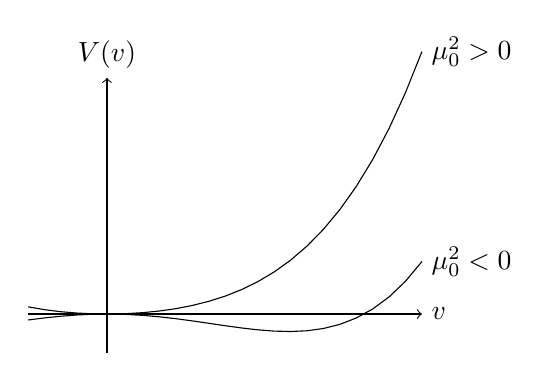
\begin{tikzpicture}
    \draw[->] (-1,0) -- (4,0) node[right] {$v$};
    \draw[->] (0,-0.5) -- (0,3) node[above] {$V(v)$};
    \draw plot[domain=-1:4] (\x,\x*\x*\x*\x/128-\x*\x/12) node[right] {$\mu_0^2<0$};
    \draw plot[domain=-1:4] (\x,\x*\x*\x*\x/128+\x*\x/12) node[right] {$\mu_0^2>0$};
\end{tikzpicture}
\caption{\label{pot}The potential used by Goldstone\cite{McGreevy:2009xe} which also is the Higgs potential. Note the minimum not being at $v=0$ giving a spontaneously broken symmetry.}
\end{figure}

\bibliographystyle{unsrt}
\bibliography{report}
\end{document}